\documentclass{amsart}
\usepackage{graphicx}
\graphicspath{{./}}
\usepackage{hyperref}
\usepackage{csvsimple}
\usepackage{longtable}
\usepackage{lscape}
\usepackage{epigraph}
\title{Zulf's Hypothesis: Asymmetric Binomial Extension of Exponential Distribution in Human Morals} 
\author{Zulfikar Moinuddin Ahmed}
\date{\today}
\begin{document}
\maketitle

\section{Search For Fundamental Model For Exponential Distribution}

We return to Simeon-Denis Poisson's original analysis of Poisson distribution (the discrete exponential) as an explanation of moral goodness in Human Race.

We make the hypothesis now that in fact underlying these is a {\em Binomial} distribution with small $p<0.5$ that gives it an exponentially decaying skew.

I better announce this model to the world.  This has a very high chance of being powerful for the Human Race Morals.

\section{Error does not dip below 0.2}

\begin{verbatim}

binom<-function(p,n,k){
  exp(log(choose(n,k))+k*log(p)+(n-k)*log(1-p))
}

bv<-function(p,n){
  z<-rep(0,10)
  for (k in 1:10){
    z[k] <- binom(p,n,k)
  }
  nrm(z) 
}

ps<-seq(0.01,0.06,by=0.001)
err<-rep(0, length(ps))
for (r in 1:length(ps)){
 z<-bv(ps[r],15)
 err[r] <- norm(y-z,type="2")
}

\end{verbatim}

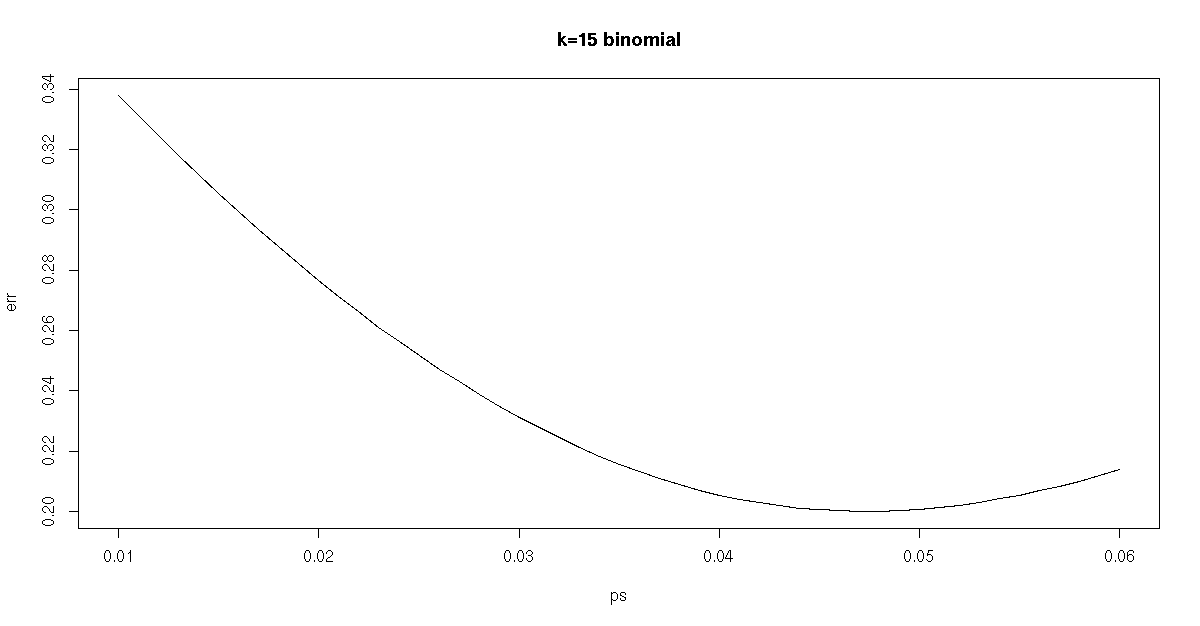
\includegraphics[scale=0.1]{error_binomial_q187.png}

\section{A Rescaled Binomial Might Work Better}

Consider a rescaled binomial distribution family as follows.  For $\alpha>0$ we consider the density $\alpha^{-1} p(x/\alpha)$. We consider $p$ an ordinary binomial.

The error is a bit better.

\section{New Hypothesis}

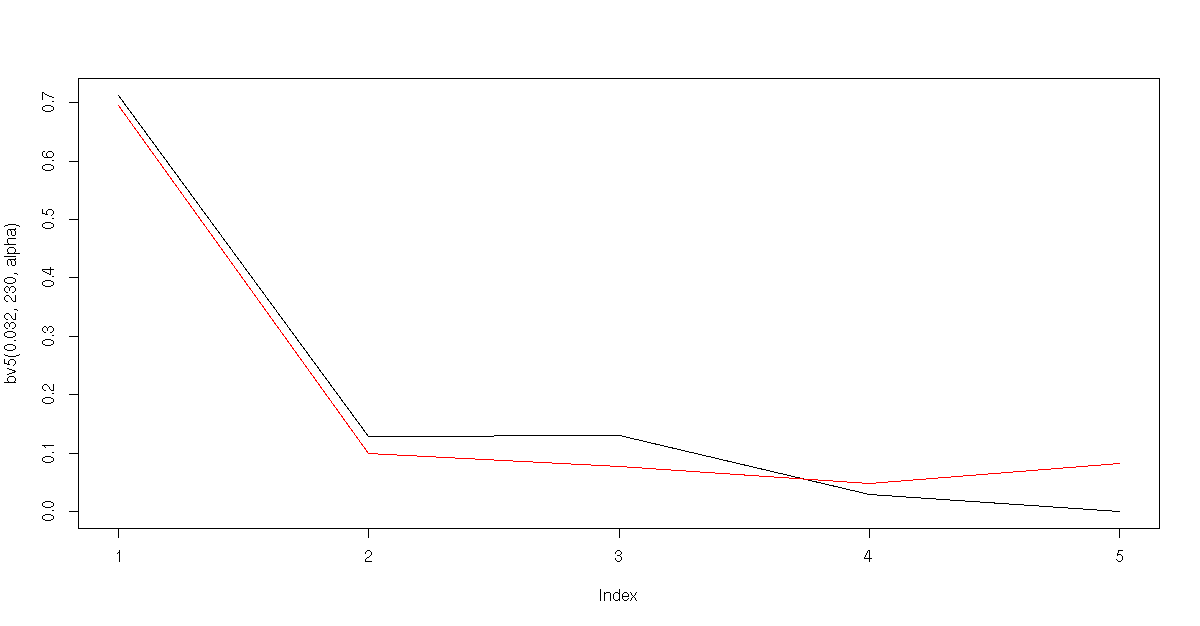
\includegraphics[scale=0.4]{scaled_binomial_fit_Q187.png}

We hypothesize three components of the data distribution.  It is a mixture of three components: (a) major component that is scaled binomial, (b) ambivalent people, (c) inverse exponential on the right end.  We're concerned mostly on left exponential I am calling 

Parameters for the left end fit above are:
\[
\alpha = 3.7
\]
and
\[
n = 230
\]
These adjust the major part of the distribution matching the first two components very well.



\end{document}